\documentclass[12pt,compress,aspectratio=169]{beamer}

\mode<presentation>
{
  \usetheme{Singapore}
  \setbeamersize{text margin left=1cm,text margin right=1cm}
%  \setbeamertemplate{navigation symbols}{} % suppress nav bar
%  \setbeamercovered{transparent}
}
\usefonttheme{professionalfonts}
\usepackage{amsmath,bm}
\usepackage{siunitx}
%\usepackage{graphicx}
\usepackage{tikz}
\usepackage{mathpazo}
\usepackage[scaled]{helvet}
\usepackage{xcolor,colortbl}
%\usepackage{hyperref}

\usetikzlibrary{decorations.pathmorphing,patterns}

\sisetup{number-math-rm=\mathnormal}

\title{Class 8: Universal Gravitation}
\subtitle{AP Physics (1, 2 and C)}
\author[TML]{Timothy Leung, Ph.D.}
\institute{Olympiads School}
\date{Fall/Winter 2017}

\newcommand{\pic}[2]{\includegraphics[width=#1\textwidth]{#2}}
\newcommand{\mb}[1]{\ensuremath\mathbf{#1}}

\begin{document}

\begin{frame}
  \maketitle
\end{frame}


\section[Intro]{Introduction}

\begin{frame}
  \frametitle{Files to Download}
  \framesubtitle{Please download/print the PDF file}
  If you have not done so already, please download the following files.
  \begin{itemize}
%  \item\texttt{00-outline.pdf}--The slightly-updated course outline
  \item\texttt{08-gravitation-print.pdf}--The ``print version'' of this week's
    slides. I recommend printing 4 slides per page.
  \item\texttt{08-Homework.pdf} This week's homework.
  \end{itemize}
\end{frame}


\begin{frame}
  \frametitle{Today's Plan}
  \begin{enumerate}
  \item Take up (some) questions from Class 7
  \item Go over this week's slides (hopefully it won't take too long)
  \end{enumerate}
\end{frame}



\section[$\mb{F}_g$]{Gravitational Force ($\mb{F}_g$)}
\begin{frame}
  \frametitle{Universal Gravitation}
  This topics we will discuss in this class are covered in AP Physics 1, 2 and
  C exams.
  \begin{itemize}
  \item Gravitational force ($\mb{F}_g$)
  \item Gravitational field ($\mb{g}$)
  \item Gravitational potential energy
  \item Kepler's laws of planetary motion
  \end{itemize}
\end{frame}


\begin{frame}
  \frametitle{Newton's Law of Universal Gravitation}
  \begin{center}
    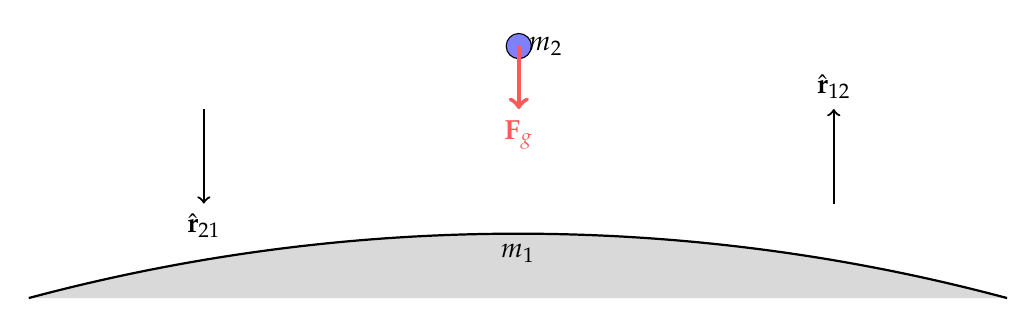
\begin{tikzpicture}[scale=0.8]
      \draw[thick,fill=gray!30] (7.75,0) arc(75:105:30)
      node[midway,below]{$m_1$};
      \draw[fill=blue!50] (0,4) circle(0.2) node[right]{$m_2$};
      \draw[ultra thick, red!65,->] (0,4)--(0,3)
      node[pos=1,below]{$\mb{F}_g$};
      \draw[->,thick](5,1.5)--(5,3) node[pos=1,above]{$\hat{\mb{r}}_{12}$};
      \draw[->,thick](-5,3)--(-5,1.5) node[pos=1,below]{$\hat{\mb{r}}_{21}$};
    \end{tikzpicture}
  \end{center}

  \vspace{-0.4in}{\Large
    \begin{displaymath}
      \boxed{
        \mb{F}_g
        =-\frac{Gm_1m_2}{r^2}\hat{\mb{r}}_{12}
        =+\frac{Gm_1m_2}{r^2}\hat{\mb{r}}_{21}
      }
    \end{displaymath}
  }

  where \fbox{$G=\SI{6.67e-11}{N.m^2/kg^2}$} is the universal gravitation
  constant, and $\hat{\mb{r}}_{12}$ and $\hat{\mb{r}}_{21}$ are
  \emph{unit vectors} (length=$1$)
\end{frame}


\begin{frame}
  \frametitle{Universal Gravitation}
  \begin{itemize}
  \item If $m_1$ exerts a gravitational force $\mb{F}_g$ on $m_2$, then $m_2$
    also exerts a gravitational force $-\mb{F}_g$ on $m_1$.
  \item The two forces are equal in magnitude and opposite in direction
    (Newton's 3rd law)
  \item Assumption: $m_1$ and $m_2$ are \emph{point masses}
    (they do not occupy any space)
  \item Therefore, for the universal gravitational equation to work:
    
    \vspace{-0.2in}{\Large
      \begin{displaymath}
        r>(r_1+r_2)
      \end{displaymath}
    }
  \end{itemize}
\end{frame}

\section[$U_g$]{Gravitational Potential Energy ($U_g$)}


\begin{frame}
  \frametitle{Gravitational Potential Energy}

  \begin{itemize}
  \item The gravitational potential energy is defined as:
    {\Large
      \begin{displaymath}
        \boxed{U_g=-\frac{Gm_1m_2}{r}}
    \end{displaymath}
    }
  %\item U_g is the work require to move two objects from $\inftypulled two objects apart, from a distance of
    % $r$ to $\infty$.
  \item It has a very similar form to the the equation for $\mb{F}_g$
  \item $U_g=0$ at $r=0$ and \emph{decrease} as $r$ decreases
  \end{itemize}
\end{frame}


\begin{frame}
  \frametitle{Relating Gravitational Potential Energy to Force}
  \begin{itemize}
  \item If you know vector calculus, you can easily see that gravitational
    force ($\mb{F}_g$) is the negative gradient of the gravitational potential
    energy ($U_g$):

    \vspace{-0.1in}{\Large
      \begin{displaymath}
        \mb{F}_g=-\nabla U_g=
        -\frac{\partial U_g}{\partial r}\hat{\mb{r}}
      \end{displaymath}
    }
  \item Even without using vector calculus, you should still see that, like
    all conservative force, $\Delta F_g=-\Delta U_g$, as we have seen in Class
    3
  \item The direction of $\mb{F}_g$ always points from high to low potential
    \begin{itemize}
    \item A falling object is always decreasing in $U_g$
    \item ``Steepest descent'': the direction of $\mb{F}$ is the shortest path
      to decrease $U_g$ 
    \item Objects traveling perpendicular to $\mb{F}$ has constant $U_g$
    \end{itemize}
  \end{itemize}
\end{frame}



%
%
%\begin{frame}
%  \frametitle{It's Very Ordinary}
%  \begin{itemize}
%  \item The governing equation for simple harmonic equation is an
%    \emph{ordinary differential equation}:
%
%    \vspace{-0.3in}{\Large
%      \begin{displaymath}
%        \boxed{\frac{d^2x}{dt^2}+\frac{k}{m}x=0}
%      \end{displaymath}
%    }
%  \item Starting with our general form, we can take the 1st and 2nd derivatives:
% 
%    \vspace{-0.35in}{\Large
%      \begin{align*}
%        x(t)&=A\sin(\omega t+\phi)\\
%        x'(t)&=A\omega\cos(\omega t+\phi)\\
%        x''(t)&=-A\omega^2\sin(\omega t+\phi)=-\omega^2x
%      \end{align*}
%    }
%    
%    \vspace{-0.2in}$\omega$ is the angular velocity, and $A$ is the amplitude,
%    and $\phi$ is a phase shift that depends on the initial condition of the
%    spring-mass system
%  \end{itemize}
%\end{frame}
%
%

%
%
%\begin{frame}
%  \frametitle{Vertical Spring-Mass System}
%  \begin{columns}
%    \column{.17\textwidth}
%    \begin{tikzpicture}[scale=1.3]
%      \node[fill=blue!70,inner sep=3.5mm] (b) at (1,2) {};
%      \draw[thick,
%        decoration={aspect=0.3,segment length=2mm, amplitude=2.5mm, coil},
%        decorate] (1,5)--(b); 
%      \fill [pattern=north east lines] (0,5) rectangle (2,5.2);
%      \draw[ultra thick] (0,5)--(2,5);
%      \draw[->](1.75,3)--(1.75,2) node[pos=1,below]{$x$};
%      \draw[very thick,->,red](b)--(1,1) node[pos=1,right]{\footnotesize $mg$};
%      \draw[very thick,->,red](b)--(1,3) node[pos=1,right]{\footnotesize $kx$};
%    \end{tikzpicture}
%    \column{.85\textwidth}
%    \begin{itemize}
%    \item For a vertical spring-mass system, the analysis is \emph{slightly}
%      more complicated (we have to consider weight as well):
%
%      \vspace{-0.2in}{\large
%        \begin{displaymath}
%          mg-kx=m\frac{d^2x}{dt^2}
%        \end{displaymath}
%    }
%    \item But since $mg$ is a constant, the only difference is the addition of a
%      constant $B$ in our expression of $x(t)$:
%    
%      \vspace{-0.35in}{\large
%        \begin{align*}
%          x(t)&=A\sin(\omega t+\phi) +B\\
%          x''(t)&=-A\omega^2\sin(\omega t+\phi)
%        \end{align*}
%      }
%    \end{itemize}
%  \end{columns}
%\end{frame}
%
%
%\begin{frame}
%  \frametitle{Vertical Spring-Mass System}
%  \begin{columns}
%    \column{.17\textwidth}
%    \begin{tikzpicture}[scale=1.3]
%      \node[fill=blue!70,inner sep=3.5mm] (b) at (1,2) {};
%      \draw[thick,
%        decoration={aspect=0.3,segment length=2mm, amplitude=2.5mm, coil},
%        decorate] (1,5)--(b); 
%      \fill [pattern=north east lines] (0,5) rectangle (2,5.2);
%      \draw[ultra thick] (0,5)--(2,5);
%      \draw[->](1.75,3)--(1.75,2) node[pos=1,below]{$x$};
%      \draw[very thick,->,red](b)--(1,1) node[pos=1,right]{\footnotesize $mg$};
%      \draw[very thick,->,red](b)--(1,3) node[pos=1,right]{\footnotesize $kx$};
%    \end{tikzpicture}
%    \column{.85\textwidth}
%    \begin{itemize}
%    \item Substituting $x(t)$ and $x''(t)$ into the differential equation gives
%
%      \vspace{-0.2in}{\Large
%        \begin{displaymath}
%          B=\frac{mg}{k}
%        \end{displaymath}
%      }
%    \item $B$ is just the stretching of the spring due to its weight
%    \item Angular velocity is the same as the horizontal case! It is still
%      given by:
%
%      \vspace{-0.35in}{\Large
%        \begin{displaymath}
%          \omega=\sqrt{\frac{k}{m}}
%        \end{displaymath}
%      }
%    \end{itemize}
%  \end{columns}
%\end{frame}
%
%
%
%\begin{frame}
%  \frametitle{Conservation of Energy in a Spring-Mass System}
%  \begin{itemize}
%  \item In both the horizontal and vertical spring-mass systems, there is no
%    friction, and so the mass and the spring form an isolated system
%  \item The forces by the spring on the mass (and by the mass on the spring)
%    are \emph{internal} forces, and energy in the system is conserved:
%
%    \vspace{-0.2in}{\Large
%      \begin{displaymath}
%        K_1 + U_{e,1} + U_{g,1} = K_2 + U_{e,2} + U_{g,2}
%      \end{displaymath}
%    }
%  \item For the horizontal spring-mass system, the total energy is:
%    
%    \vspace{-0.2in}{\Large
%      \begin{displaymath}
%        E_\mathrm{total}=\frac{1}{2}kA^2
%      \end{displaymath}
%   }
%  \end{itemize}
%\end{frame}
%
%
%%\begin{frame}
%%  \frametitle{What if It's Not Perfect}
%%  \begin{itemize}
%%  \item A \emph{damped harmonic system} is when there is frictional losses
%%  \end{itemize}
%%\end{frame}
%
%
%\begin{frame}
%  \frametitle{Simple Example}
%  \textbf{Example 2:} A mass suspended from a spring is oscillating up and
%  down. Consider the following two statements:
%  \begin{enumerate}
%  \item At some point during the oscillation, the mass has zero velocity but it
%    is accelerating
%  \item At some point during the oscillation, the mass has zero velocity and
%    zero acceleration.
%  \end{enumerate}
%
%  \begin{enumerate}[(a)]
%  \item Both occur at some time during the oscillation
%  \item Neither occurs during the oscillation
%  \item Only (1) occurs
%  \item Only (2) occurs
%  \end{enumerate}
%\end{frame}
%
%
%
%\begin{frame}
%  \frametitle{Another Example}
%  \textbf{Example 3:} An object of mass \SI{5}{\kg} hangs from a spring and
%  oscillates with a period of \SI{0.5}{\second}. By how much will the
%  equilibrium length of the spring be shortened when the object is removed.
%  \begin{enumerate}[(a)]
%  \item\SI{0.75}{\centi\metre}
%  \item\SI{1.50}{\centi\metre}
%  \item\SI{3.13}{\centi\metre}
%  \item\SI{6.20}{\centi\metre}
%  \end{enumerate}
%\end{frame}



\section[$\mb{g}$]{Gravitational Field ($\mb{g}$)}


\begin{frame}
  \frametitle{Gravitational Field}
  \framesubtitle{A Review}
%  \begin{columns}
%    \column{0.75\textwidth}
  \begin{itemize}
  \item The concept of gravitational field was studied in Grade 12 Physics, so
    this \emph{should} be a review
%  \item A condensed copy of my notes/slides for Physics 12 
%    \item For a pendulum, there are two forces acting on the mass: weight
%      $F_g=mg$ and tension $T$
%    \item When the mass is deflected by an angle $\theta$, it's easy to show
%      (using polar coordinates) that the force in the angular direction is
%      $F_\theta=-mg\sin\theta$
%    \item We needn't worry about the radial direction because it doesn't
%      have anything to do with the restoring force
  \end{itemize}
%
%    \column{0.25\textwidth}
%    \begin{tikzpicture}
%      \fill[pattern=north east lines] (-1,0) rectangle (1,0.2);
%      \draw[very thick](-1,0)--(1,0);
%      \begin{scope}[rotate=10]
%        \draw[thick](0,0)--(0,-5);
%        \tikzstyle{balloon}=[ball color=red];    
%        \shade[balloon] (0,-5) circle (0.2) node[below right]{$m$};
%        \draw[dotted,->,very thick,red](0,-5)--(-0.5,-5)
%        node[pos=1,left]{\footnotesize $mg\sin\theta$};
%        \draw[->,very thick,red](0,-5)--(0,-3)
%        node[pos=1,left]{\footnotesize $T$};
%        \draw[->,very thick,red, rotate around={-10:(0,-5)}](0,-5)--(0,-6.5)
%        node[pos=1,below]{\footnotesize $F_g$};
%      \end{scope}
%      \draw[dashed,thin](0,0)--(0,-5);
%      \draw[->](0,-2) arc(270:280:2) node[pos=0.5,below]{$\theta$};
%    \end{tikzpicture}
%  \end{columns}
\end{frame}


\begin{frame}
  \frametitle{Think Gravitational Field: What is $g$?}
  \begin{itemize}
  \item We generally describe the force of gravity as

    \vspace{-.25in}{\Large
      \begin{displaymath}
        \mb{F}_g=m\mb{g}
      \end{displaymath}
    }
  \item To find the magnitude of $g$, we group the variables in Newton's
    universal gravitation equation:
    
    \vspace{-.3in}{\Large
      \begin{displaymath}
        F_g=\underbrace{\left[\frac{Gm_1}{r^2}\right]}_{=g}m_2=m_2g
      \end{displaymath}
    }
  \item On the surface of Earth, we use use $m_1=m_\mathrm{Earth}$ and
    $r=r_\mathrm{Earth}$ to compute $g=\SI{9.81}{m/s^2}$, or $g=\SI{9.81}{N/kg}$
    (both units are  equivalent)
%  \item Farther away from Earth's surface, however, $r$ increases and $g$
%    decreases
%  \item $\mb{g}$ is known as the \textbf{gravitational field}
  \end{itemize}
\end{frame}

\begin{frame}
  \frametitle{Gravitational Field}

  \begin{itemize}
  \item The intensity of the \textbf{gravitational field} $\mb{g}$ generated by
    a source mass $m_s$ is defined by:

    \vspace{-0.3in}{\Large
      \begin{displaymath}
        \boxed{g(m_s,r)=\frac{Gm_s}{r^2}}
      \end{displaymath}
    }
%  \item Not a constant
%  \item Covers all space around point mass $m_s$
  \item Mapping of how $m_s$ influences the gravitational forces on other masses
%    
%    \vspace{-0.2in}{\Large
%      \begin{displaymath}
%        \mb{F}_g=m\mb{g}
%      \end{displaymath}
%    }
%
  \end{itemize}

  \vspace{-0.1in}
  \begin{center}
    \begin{tabular}{l|c|c}
      \rowcolor{pink}
      \textbf{Quantity} & \textbf{Symbol} & \textbf{SI Unit} \\ \hline
      Gravitational field intensity    & $g$   & \si{N/kg}\\
      Universal gravitational constant & $G$   & \si{N.m^2/kg^2} \\
      Mass of source (a point mass)    & $m_s$ & \si{kg} \\
      Distance from centre of source   & $r$   & \si{m} \\
    \end{tabular}
  \end{center}
\end{frame}


\begin{frame}
  \frametitle{Relating Gravitational Field \& Gravitational Force}
  \begin{itemize}
  \item $\mb{g}$ itself doesn't do anything until there is another mass $m$.
    At which point, $m$ experiences a gravitational force  related to $\mb{g}$
    by:

    \vspace{-0.2in}{\Large
      \begin{displaymath}
        \boxed{\mb{g}=\frac{\mb{F}_g}{m}}
      \end{displaymath}
    }
  \item $\mb{F}_g$ and  $\mb{g}$ are vectors in the same direction: toward the
    centre of the source mass that created the field, therefore all vector
    operations apply
  \end{itemize}

  \begin{center}
    \begin{tabular}{l|c|c}
      \rowcolor{pink}
      \textbf{Quantity} & \textbf{Symbol} & \textbf{SI Unit} \\ \hline
      Gravitational field & $\mb{g}$   & \si{N/kg}\\
      Gravitational force on a mass & $\mb{F}_g$ & \si{N} \\
      Mass inside the gravitational field & $m$ & \si{kg} \\
    \end{tabular}
  \end{center}
\end{frame}

%\begin{frame}
%  \frametitle{Example Problem}
%  \textbf{Example 1:} Calculate the gravitational field intensity at a height
%  of $300.0km$ from Earth's surface.\\
%  \begin{center}
%    \pic{.65}{graphics/ISS02_NASA_4288.jpg}
%  \end{center}
%  Remember, gravitational field intensity is the same as acceleration due to
%  gravity at that point!
%\end{frame}
%
%
\begin{frame}
  \frametitle{Relating $U_g$, $\mb{F}_g$ and $\mb{g}$}
  \begin{itemize}
  \item Knowing that $\mb{F}_g$ and $\mb{g}$ only differ by a constant, we can
    also relate gravitational field to $U_g$ by the gradient operator:

    \vspace{-0.1in}{\Large
      \begin{displaymath}
        \mb{g}=\frac{\mb{F}_g}{m}=-\nabla\left(\frac{U_g}{m}\right)=
        -\frac{\partial}{\partial r}\left(\frac{U_g}{m}\right)
        \hat{\mb{r}}
      \end{displaymath}
    }
  \item We already know that the direction of $\mb{g}$ is the same as
    $\mb{F}_g$, i.e.\
    \begin{itemize}
    \item The direction of $\mb{g}$ is the shortest path to decrease $U_g$ 
    \item Objects traveling perpendicular to $\mb{g}$ has constant $U_g$
    \end{itemize}
  \end{itemize}
\end{frame}


\begin{frame}
  \frametitle{Gravitational Field Lines}
  \begin{center}
    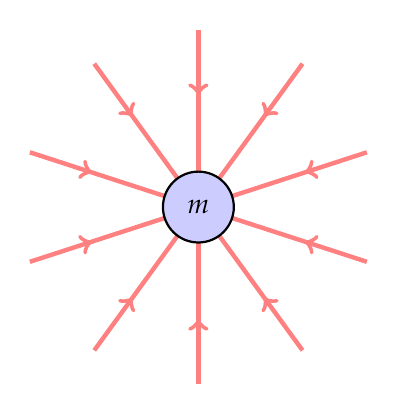
\begin{tikzpicture}[scale=1.5]
      \foreach \x in {0,...,9}\draw[red!50,ultra thick,rotate=36*\x](0,0)--(0,1);
      \foreach \x in {0,...,9}\draw[red!50,<-,ultra thick,rotate around={36*\x:(0,0)}](0,0.95)--(0,1.5);
      \draw[fill=blue!20,thick](0,0) circle(0.3) node{$m$};
    \end{tikzpicture}
  \end{center}
  \begin{itemize}
  \item The direction of $\mb{g}$ is towards the centre of the object that
    created it
  \item Field lines do not tell the intensity (i.e.\ magnitude) of $\mb{g}$,
    only the direction
  \end{itemize}
\end{frame}



\section{Orbital Motion}

\begin{frame}
  \frametitle{Orbital Speed}
  \framesubtitle{Newton's Thought Experiment}
  \begin{center}
    \pic{1}{figure-5.jpg}
  \end{center}

  \vspace{-.3in}So how fast is fast enough?
\end{frame}


\begin{frame}
  \frametitle{Orbital Speed}
  \framesubtitle{Relating Gravitational and Centripetal Force}
  \begin{itemize}
%  \item The velocity required for an object to reach an orbital path without
%    falling back onto the surface. For example:
%    \begin{itemize}
%    \item A spy satellite orbiting around Earth
%    \item The moon orbiting around Earth
%    \item The Earth orbiting around the Sun
%    \end{itemize}
  \item Assume a circular orbit (since we know it best)
  \item The centripetal force (required force) is equal to the gravitational
    force (supplied force):

    \vspace{-0.3in}{\Large
      \begin{displaymath}
        \underbrace{\frac{GMm}{r^2}}_\mathrm{F_g}
        =\underbrace{\frac{mv^2}{r}}_\mathrm{F_c}
      \end{displaymath}
    }
    where $r$ is the distance between the centres of the two objects
  \end{itemize}
\end{frame}

\begin{frame}
  \frametitle{Orbital Speed}
  \begin{itemize}
  \item Cancelling $m$, and $r$ in both sides of the equation, and solving for
    $v$, we get:
    
    \vspace{-0.15in}{\Large
      \begin{displaymath}
        \boxed{v_\mathrm{orbit}=\sqrt{\frac{GM}{r}}}
      \end{displaymath}
    }
  \item Orbital speed $v_\mathrm{orbit}$ is sometimes also called orbital
    velocity
  \item Does not depend on the mass of the object in orbit
  \item A $\SI{1.5e-13}{\kg}$ speck of cosmic dust and the $\SI{419600}{\kg}$
    International Space Station both have the same $v_\mathrm{orbit}$ around
    Earth if they are at the same altitude
  \end{itemize}
\end{frame}


\begin{frame}
  \frametitle{Escape Speed}
  An object can leave the surface of Earth at any speed. But when all the
  kinetic energy of that object is converted to gravitational potential, it'll
  return back to the surface of the earth. There is, however, a \emph{minimum}
  velocity at which the object \emph{would not} fall back to Earth because of
  gravity.
\end{frame}


\begin{frame}
  \frametitle{Escape Speed}
  \begin{itemize}
  \item The gravitational potential energy of an object with mass $m$ on the
    surface of a planet (with mass $M$ and radius $r$) is

    \vspace{-0.15in}{\Large
      \begin{displaymath}
        U_g=-\frac{GMm}{r}
      \end{displaymath}
    }
  \item The most amount of work that you can do is to bring it to the other side
    of the universe $r=\infty$, where $U_g=0$.
  \item If you start with \emph{more} kinetic energy than required to do all
    the work, then the object has \emph{escaped} the gravitational pull of the
    planet.
  \end{itemize}
\end{frame}


\begin{frame}
  \frametitle{Escape Speed}
  \begin{itemize}
  \item Set $K$ to equal to $-U_g$:
    
    \vspace{-0.2in}{\Large
      \begin{displaymath}
        \frac{1}{2}mv^2=\frac{GMm}{r}
      \end{displaymath}
    }
  \item We can then solve for escape speed $v=v_\mathrm{esc}$:

    \vspace{-0.2in}{\Large
      \begin{displaymath}
        \boxed{v_\mathrm{esc}=\sqrt{\frac{2GM}{r}}}
      \end{displaymath}
    }

  \item There is a simple relationship between orbital speed and escape
    speed:

    \vspace{-.2in}{\Large
      \begin{displaymath}
        \boxed{v_\mathrm{esc}=\sqrt{2} v_\mathrm{orbit}}
      \end{displaymath}
    }
    %For any $v>v_\mathrm{esc}$ the object can break free of a planet's 
    %gravitational pull.
  \end{itemize}
\end{frame}


\begin{frame}
  \frametitle{What if I'm not escaping from the surface?}
  \begin{itemize}
  \item These two situations have the same escape speed:
    \begin{center}
      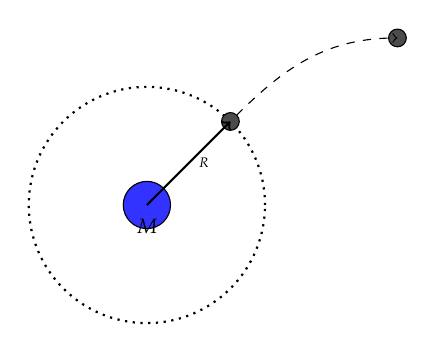
\begin{tikzpicture}[scale=1.5]
        \draw[fill=blue!80](0,0) circle(0.2) node[midway,below]{\tiny $M$};
        \draw[dotted,thick] (0,0) circle(1);
        \begin{scope}[rotate around={45:(0,0)}]
          \draw[fill=black!70](1,0) circle(0.075);
          \draw[->,thick](0,0)--(1,0) node[midway,right]{\tiny $R$};
          \draw[fill=black!70](2.5,-0.5) circle(0.075);
          \draw[->,dashed](1.075,0) to[out=0,in=135](2.5,-0.5);      
        \end{scope}
      \end{tikzpicture}
      \hspace{0.2in}
      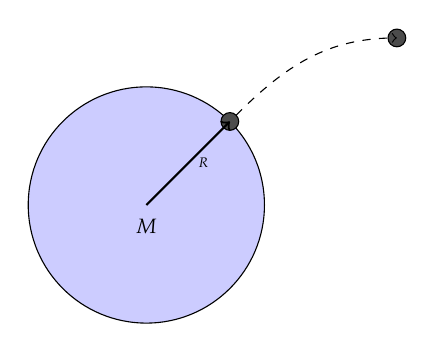
\begin{tikzpicture}[scale=1.5]
        \draw[fill=blue!20] (0,0) circle(1) node[midway,below]{\tiny $M$};
        \begin{scope}[rotate around={45:(0,0)}]
          \draw[fill=black!70](1,0) circle(0.075);
          \draw[->,thick](0,0)--(1,0) node[midway,right]{\tiny $R$};
          \draw[fill=black!70](2.5,-0.5) circle(0.075);
          \draw[->,dashed](1.075,0) to[out=0,in=135](2.5,-0.5);      
        \end{scope}
      \end{tikzpicture}
    \end{center}

  \item The only difference is that an object already in orbit (left figure)
    already has orbital speed $v_\mathrm{orbit}$, so escaping from that orbit
    requires an additional speed of

    \vspace{-0.45in}{\Large
      \begin{displaymath}
        \Delta v=v_\mathrm{esc}-v_\mathrm{orbit}
      \end{displaymath}
    }
  \end{itemize}
\end{frame}


\begin{frame}
  \frametitle{Orbital Energies}
  \begin{itemize}
  \item We can obtain the \textbf{orbital kinetic energy} by using the orbital
    speed in our expression of kinetic energy:

    \vspace{-.35in}{\Large
      \begin{displaymath}
        K_\mathrm{orbit}=\frac{1}{2}mv_\mathrm{orbit}^2=\frac{1}{2}m
        \left(\sqrt{\frac{GM}{r}}\right)^2=\boxed{\frac{GMm}{2r}}
      \end{displaymath}
    }
  \item And we already have an expression for
    \textbf{gravitational potential energy}:

    \vspace{-0.15in}{\Large
      \begin{displaymath}
        U_g=-\frac{GMm}{r}=-2K_\mathrm{orbit}
      \end{displaymath}
    }
  \item\textbf{Total orbital energy} is the sum of $K$ and $U_g$!

    \vspace{-0.15in}{\Large
      \begin{displaymath}
        E_T=K+U_g=-\frac{GMm}{2r}=-K_\mathrm{orbit}
      \end{displaymath}
      }
  \end{itemize}
\end{frame}


\begin{frame}
  \frametitle{Kepler's Law of Planetary Motion}
%  \textbf{Example 5:} A bucket full of water is attached to a rope and allowed
%  to swing back and forth as a pendulum from a fixed support. The bucket has a
%  hole in its bottom that allows water to leak out. How does the period of
%  motion change with the loss of water?
%  \begin{enumerate}[(a)]
%  \item The period does not change.
%  \item The period continuously decreases.
%  \item The period continuously increases.
%  \item The period increases to some maximum and then decreases again.
%  \end{enumerate}
\end{frame}


%\begin{frame}
%  \frametitle{Think About $g$}
%  \textbf{Example 6:} A little girl is playing with a toy pendulum while riding
%  in an elevator. Being an astute and educated young lass, she notes that the 
%  period of the pendulum is $T=\SI{0.5}{\second}$. Suddenly the cables
%  supporting the elevator break and all  of the brakes and safety features fail
%  simultaneously. The elevator plunges into free fall. The young girl is
%  astonished to discover that the pendulum has:
%  \begin{enumerate}[(a)]
%  \item continued oscillating with a period of \SI{0.5}{\second}.
%  \item stopped oscillating entirely.
%  \item decreased its rate of oscillation to have a longer period.
%  \item increased its rate of oscillation to have a lesser period.
%  \end{enumerate}
%\end{frame}

\section{Gravitational Potential Energy}


\end{document}
